\subsection{Prueba \#2 :}
Evalue el resultado de las dos funciones implementadas anteriormente con este conjunto de datos:\\

\doublebox{
    \begin{minipage}[c][1.2\height] [c]{1\textwidth}
var data = [\newline
[40 ,70] ,\newline
[70 ,130] ,\newline
[90 ,40] ,\newline
[110 , 100] ,\newline
[140 ,110] ,\newline
[160 , 100] ,\newline
[150 , 30]\newline
];\newline
var point = [140 ,90]; // query
    \end{minipage}
}
\begin{figure}[H]
 \centering
 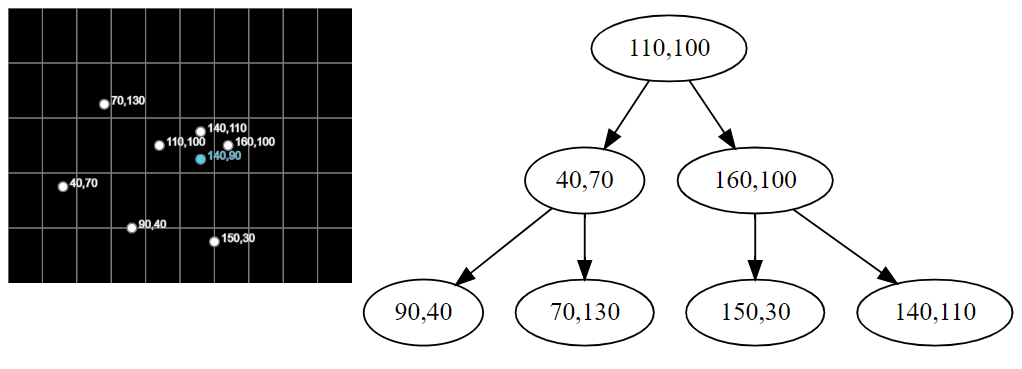
\includegraphics[width=0.9\textwidth]{images/prueba2.PNG}
 \label{fig:act-5-prueba2}
\end{figure}

\begin{itemize}
    \item closest\_point\_brute\_force
    \begin{figure}[H]
     \centering
     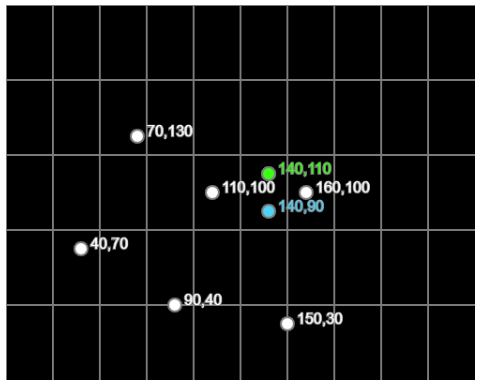
\includegraphics[width=0.5\textwidth]{images/prueba2_brute_force.PNG}
     \label{fig:act-6-1}
     \caption{Podemos apreciar el punto mas cercano de color \textcolor{green}{verde} el cual es [140,110].}
    \end{figure}
    \item naive\_closest\_point
    \begin{figure}[H]
     \centering
     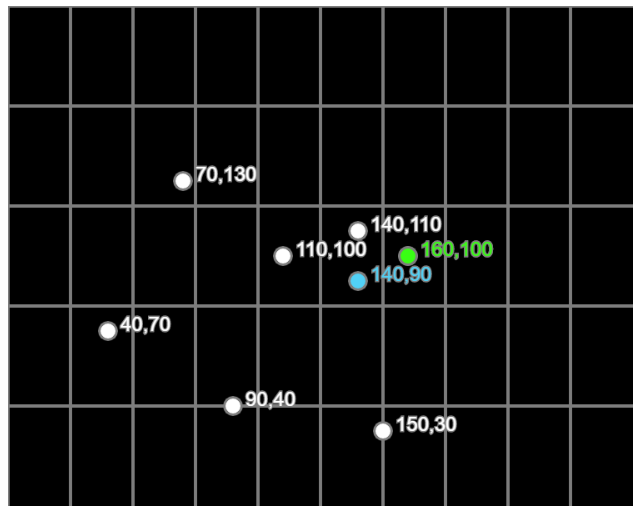
\includegraphics[width=0.6\textwidth]{images/prueba2_naive.PNG}
     \label{fig:act-6-2}
     \caption{Podemos apreciar el punto mas cercano de color \textcolor{green}{verde} el cual es [160,100].}
    \end{figure}
\end{itemize}

Observamos que en la función closest\_point\_brute\_force el punto mas cercano es [140,110] y en naive\_closest\_point el punto mas cercano es [160,100].


